\chapter{Artificial Neural Networks}
\section{Artificial Neuron}
Our brain is composed by biological neurons and an artificial neuron (or AN) is a representation of it. Every AN can gather signals from other neurons or from the environment, and after an elaboration it transmits another signal to all the other ANs that are connected to it \cite{engelbrecht2007computational}. A rapresentation of AN is depicted in \ref{fig:artificial_neuron}. \\
Each connection to the artificial neuron has a numerical weigth associated to it in which the input signal is hold back. The value of the weight can be either positive or negative. In most cases, the sums of each node are weighted and then given as input to a \textit{non-linear} function called \textbf{transfer function} or \textbf{activation function} \cite{artificial_neuron_wiki}. The activate function defines the output value of the node and typically, the \textit{Step Function}, \textit{Sigmoid Function} and a \textit{Softmax Function} are the most used.

\begin{figure}[!ht]
    \centering
    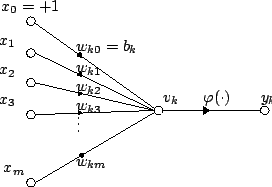
\includegraphics[scale=0.5]{Figures/artificial_neuron.png}
    \caption{Representation of an Artificial Neuron \cite{artificial_neuron_wiki}}
    \label{fig:artificial_neuron}
\end{figure}

\noindent From the mathematical point of view, we can define an artificial neuron as follow: \\
given $m+1$ inputs with signals from $x_1$ to $x_m$ and weights values from $w_0$ to $w_m$. The \textit{bias} is then defined by the input $x_0$ in which a value of 1 will be assigned. The bias value allows us to \textit{shift} the curve of the activation function to a certain direction and it is defined with $w_{k0} = b_k$ \cite{artificial_neuron_wiki}. \\
The output of the AN is:

\begin{equation*}
    y_k = \varphi \left ( \sum_{j=0}^{m} w_{kj} x_j \right )
\end{equation*}

\section{Network Function}
When there are many aritificial neurons interconnected between each other in the different layers, we form a \textit{network}. \ref{fig:ann} shows an example of ANN where the \textbf{inputs} are represented by the first layer in which they send data through the connection to the second group of neuron. The connection between two neuros is called \textit{synapses} where the \textbf{weigth} is stored. The second layer is connected to the third one that represents the \textbf{output} of the network. There can be multiple stratums between the inputs and the outputs and these are called \textit{hidden layers}. \\

\begin{figure}[!ht]
    \centering
    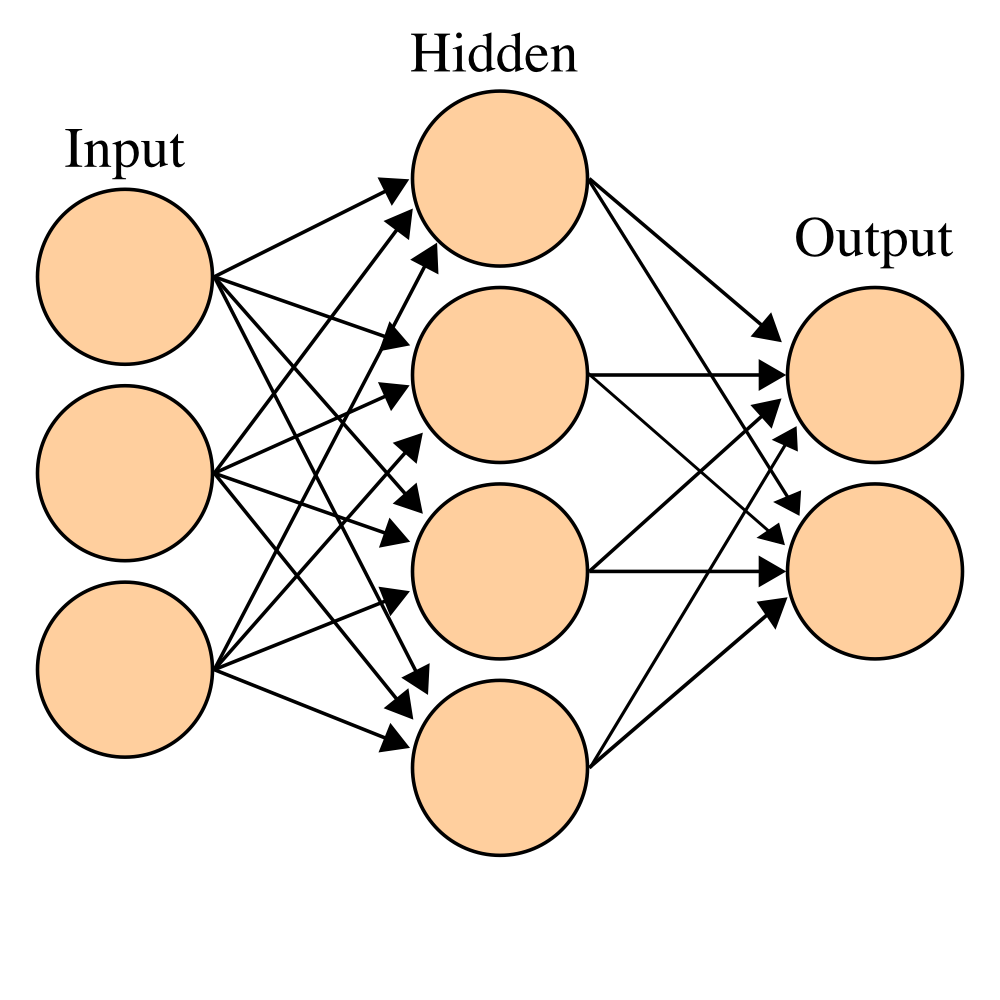
\includegraphics[scale=0.15]{Figures/ann.png}
    \caption{Example of ANN \cite{ann_wiki}}
    \label{fig:ann}
\end{figure}

\vspace*{0.33in}

\noindent Typically, a neural network is defined by three factors:
\begin{itemize}
    \item[1] How the different layers are interconnected
    \item[2] How the the weights are updated (learning process)
    \item[3] How the neuron's input value is converted to its output activation (activation function)
\end{itemize}

\section{Learning}
For every application the design of a neural network is different and after it has structured, the NN is ready to be trained. The first step is the initialization of the weigths. Normally they are initialized with random values, although, in \cite{yam2000weight} they developed a method to \textit{``determining the optimal initial weights of feedforward neural networks based on the Cauchy's inequality and a linear algebraic method''}. More, in \cite{fernandez2001weight} they tested seven different weights' initialization for twelve different problems. Thus, even the initialization of the connections values is application-dependant. \\
\noindent The learning paradigms can be grouped in three major categories: \textbf{supervised}, \textbf{unsupervised} and \textbf{reinforcement learning}.

\subsubsection{Supervised Learning}
This learning technique is the task of inferring a function from labeled training data \cite{sup_learn_wiki} \cite{mohri2012foundations}. The set responsible for training the model is composed by \textit{training examples} in which every sample consists of an \textit{input object} and a \textbf{desidered} \textit{output value}. What the algorithms does is to analyze the train dataset and produce an inferred function that will be used to map the new examples \cite{sup_learn_wiki}. Basically, the algorithm can be seen as \textit{learning} with a \textit{teacher}, in the sense that the there is costantly a feedback on the status of the application.

\subsubsection{Unsupervised Learning}
While in supervised learning, the system has a desidered output given from the training dataset, in the unsupervised paradigm, the system has to learn to estimate the right output given a new input \cite{ghahramani2004unsupervised}. In \textit{classification}, this output is a class label whereas in \textit{regression} is a real number. There are several ways to model this kind of learning system. \textit{Clustering}, using \textit{Self-Organizing Maps}, \textit{K-means} or \textit{hierachical clustering} are among the most famous approaches.

\subsubsection{Reinforcement Learning}
In reinforcement learning, the system takes actions to interact with its own environment. Each action will affect the state of the environment in which will produe a result in a form of either \textit{reward} or \textit{punishment}. The goal of this learning paradigm is to learn which is the best sequence of actions that maximises the rewards or minimises the punishments. There are quite a few approaches to find the best sequence of actions. The most famouse are \textit{Monte Carlo methods}, \textit{Temporal Difference methods} and \textit{Direct Policy search methods}.

\section{Multilayer Perceptron}
The model created by the Multilayer perceptron (MLP) serves to map a set of inputs onto a group of ouputs. The main feature of the MLP is that it a \textit{feedforward} artificial neural network. The MLP is formed by a defined number or layers in which every layer is \textit{fully connected} to following one. Every neuron of the network has a nonlinear activation function, with the exception of the input nodes. The techinque used in the MLP is of the kind of supervised and it uses the \textbf{backpropagation} for training the neurons \cite{mlp_wiki}. Backpropagation is discussed more in details in \ref{ssec:backprop}.

\subsubsection{Learning through Backpropagation} \label{ssec:backprop}
The learning phase in the neural network occurs in the moment that the connection weigths change based on the error value in the output. The error is calculated comparing the result the network produced with the expected one. This is a typical example of supervised learning because the network compares the result it just obtained with the one that it was expecting. This process is done through \textbf{backproagation}. \\

\noindent In backpropagation, the error output of the node $j$ in the $nth$ sample of the training dataset is given by
\begin{equation}
    e_{j}(n) = d_{j}(n) - y_{j}(n)
\end{equation}
where $d$ is the expected output whereas $y$ is the output value obtained from the neuron. The weights are then adjusted in such a way that the error is minimized. With \ref{eq:output_error} we are able to determine the corrections to apply given an output value produced by a perceptron.

\begin{equation}\label{eq:output_error}
    \varepsilon (n) = \frac{1}{2}\sum_{j} e^2_{j}(n)
\end{equation}

\noindent At this point using \ref{eq:gradient} we are able to determine the amount of change for each weight. This is done by \textbf{gradient descent} which is a first-order optimization algorithm. Gradient descent is used to find \textit{local minima} of a function, where \textit{"it takes steps proportionally to the negative of the gradient of the function in that point"}\cite{gradient_wiki}. The opposite instead, it means that it is approaching to the \textit{local maxima} of the function. ALthough, in this way, the process would be called \textit{gradient ascent}\cite{gradient_wiki}.

\begin{equation}\label{eq:gradient}
    \Delta w_{ji}(n) = -\eta \frac{\partial \varepsilon (n)}{\partial v_{j} (n)}y_{j}(n)
\end{equation}

\noindent In \ref{eq:gradient}, $\eta$ represents the \textit{learning rate} whereas $y_{i}$ is the output of the previous neuron \cite{mlp_wiki}. The learning rate parameter is one of the most importan parameters when design a neural network. The reason is that, the value used for it ensures that the weights are converging as fast as possible avoiding waivings. \\

\noindent The calculation of the derivates depends on the field $v_{j}$ where this value changes itself. Continuing, \ref{eq:gradient} can be simplified to \ref{eq:simpl_gradient} where $\phi^{\prime}$ represents the \textit{derivate} of the activation function described before. Note that this does not changes itself.

\begin{equation}\label{eq:simpl_gradient}
    \frac{\partial \varepsilon (n)}{\partial v_{j} (n)} = e_{j}(n)\phi^{\prime}(v_{j}(n))
\end{equation}

\section{Deep Learning}
\label{sec:deep_learning}
Deep Learning has several definitions in which those have been changing in last 10 years. Definition number 5 reported in \cite{deng2014deep} says the following: \textit{"Deep Learning is a new area of Machine Learning research, which has been introduced with the objective of moving Machine Learning closer to one of its original goals: Artificial Intelligence. Deep Learning is about learning multiple levels of representation and abstraction that help to make sense of data such as images, sound, and text."}.

\noindent There are two main aspects of the level of representations described above:
\begin{itemize}
    \item[1)] a model consists of several layers of nonlinear processing units
    \item[2)] for supervised and unsupervised approaches the feature representation have more abstract layers
\end{itemize}
\noindent It is possible to classify Deep Learning as an intersection between different research areas, such as: neural networks, pattern recognition, signal processing, etc..\cite{deng2014deep}

\subsection{Deep Neural Networs}
As described in \ref{sec:deep_learning}, a \textit{deep neural network} is composed by several hidden layers of perceptrons between the input(s) and the output(s) \cite{bengio2009learning}. As for the artificial neural networks, DNNs are able to model complex non-linear relationships. \cite{deep_learning_wiki}

\noindent Adding extra layers to a ANN permits to each layer to \textit{specialize} in solving a certain problem. For example, in \textit{visual pattern recognition} the neurons in the first layer can try to learn how to recognize edges in a picture, whereas those in the second layer might focus in learning ho to recognize more complex shapes like a square or a triangle built up from the previous edges. The next layers will try to learn even more complex shapes. In the case of speech recognition, we could split the problem in different parts as well. The first layer could focus in recognizing phonemes, the second layer can learn about the pitch voice, and so on.

\noindent The usage of multiple hidden layers gives to DNNs some advantages in learning how to solve complex problems compared to the shallow networks.\cite{dnn_website} An example of DNN is depicted in \ref{fig:deep_nn}.

\begin{figure}[!ht]
    \centering
    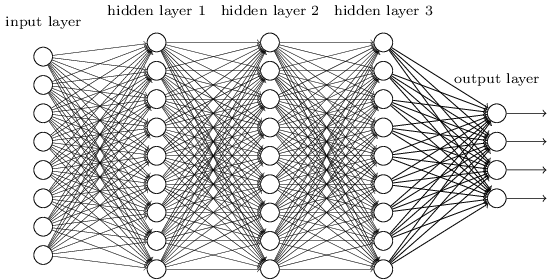
\includegraphics[scale=0.6]{Figures/deep_nn.png}
    \caption{Example of Deep Neural Network \cite{dnn_website}}
    \label{fig:deep_nn}
\end{figure}

\subsubsection{Architecture}
Deep Neural Networks are oftenly designed as feedforward networks and trained with the \textit{back propagation} algorithm. Although, to train acoustinc models for Automatic Speech Recognition (ASR) \textit{Convolutional Deep Neural Networks} (CNNs) presented better results than the typical feedforward design. Despite the similarity between the two networks, in CNNs \textit{"the neurons in the inputs of hidden units in layer m are from a subset of units in layer m-1, units that have spatially contiguous receptive fields"}. \cite{lenet}

\noindent To update the weights the \textit{stochastic gradient descent} is used as follow:

\begin{equation}
    w_{ij}(t+1) = w_{ij}(t) + \eta  \frac{\partial C}{\partial w_{ij}}
\end{equation}

\noindent where $\eta$ is the \textit{learning rate} whereas  $C$ is the \textit{cost function}. The activation function and the learning type have a direct influence in the choice of the cost function. For instance, a typical choice of the activation function for a supervised learning approach on a problem of multiclass classification are either \textbf{softmax function} or \textbf{cross entropy function}. The mathematical definition of \textit{softmax function} is defined in \ref{eq:softmax} where $p_{j}$ represents the class probability whereas $x_{k}$ and $x_{j}$ are the total input to neuron $x$ and $j$ of that layer. \textit{Cross entropy function} is defined by \ref{eq:cross_entropy} where $d_{j}$ is the target probability of the output neurons $j$ and $p_{j}$ is the probability output for $j$ after applying the activation function. \cite{deep_learning_wiki}

\begin{equation}\label{eq:softmax}
    p_{j} =  \frac{exp(x_{j})}{ \sum_k exp(x_{k})}
\end{equation}
\begin{equation}\label{eq:cross_entropy}
    C = -\sum_j d_{j}log(p_{j})
\end{equation}
